
\chapter{Experimental Setup}

This chapter describes the experimental setup used in this study, for the sake of brevity, it is provided a brief descriptions of the Large Hadron Collider (LHC), the Compact Muons Solenoid (CMS), and its subdetectors, and the process of high-level physics objects processing and reconstruction.

\section{The Large Hadron Collider}
\todo[inline]{FAZER!}

The Large Hadron Collider (LHC) is the world largest and powerful particle accelerator for protons and heavy-ions ever build. It is located in a complex of other accelerator operated by the European Organization for Nuclear Research (CERN), in the border of between Switzerland and France. The LHC is built in the same 27 km extension tunnel once used by Large Electron–Positron Collider. The CERN complex is a composition of many accelerators, for proton and heavy-ions, used to provide beams of particles for smaller experiments and as a sequence of injectors for the LHC. Figure~\ref{lhc_complex} presents the many components of the LHC complex of accelerators.

% lhc complex
\begin{figure}[htbp]
    \centering
    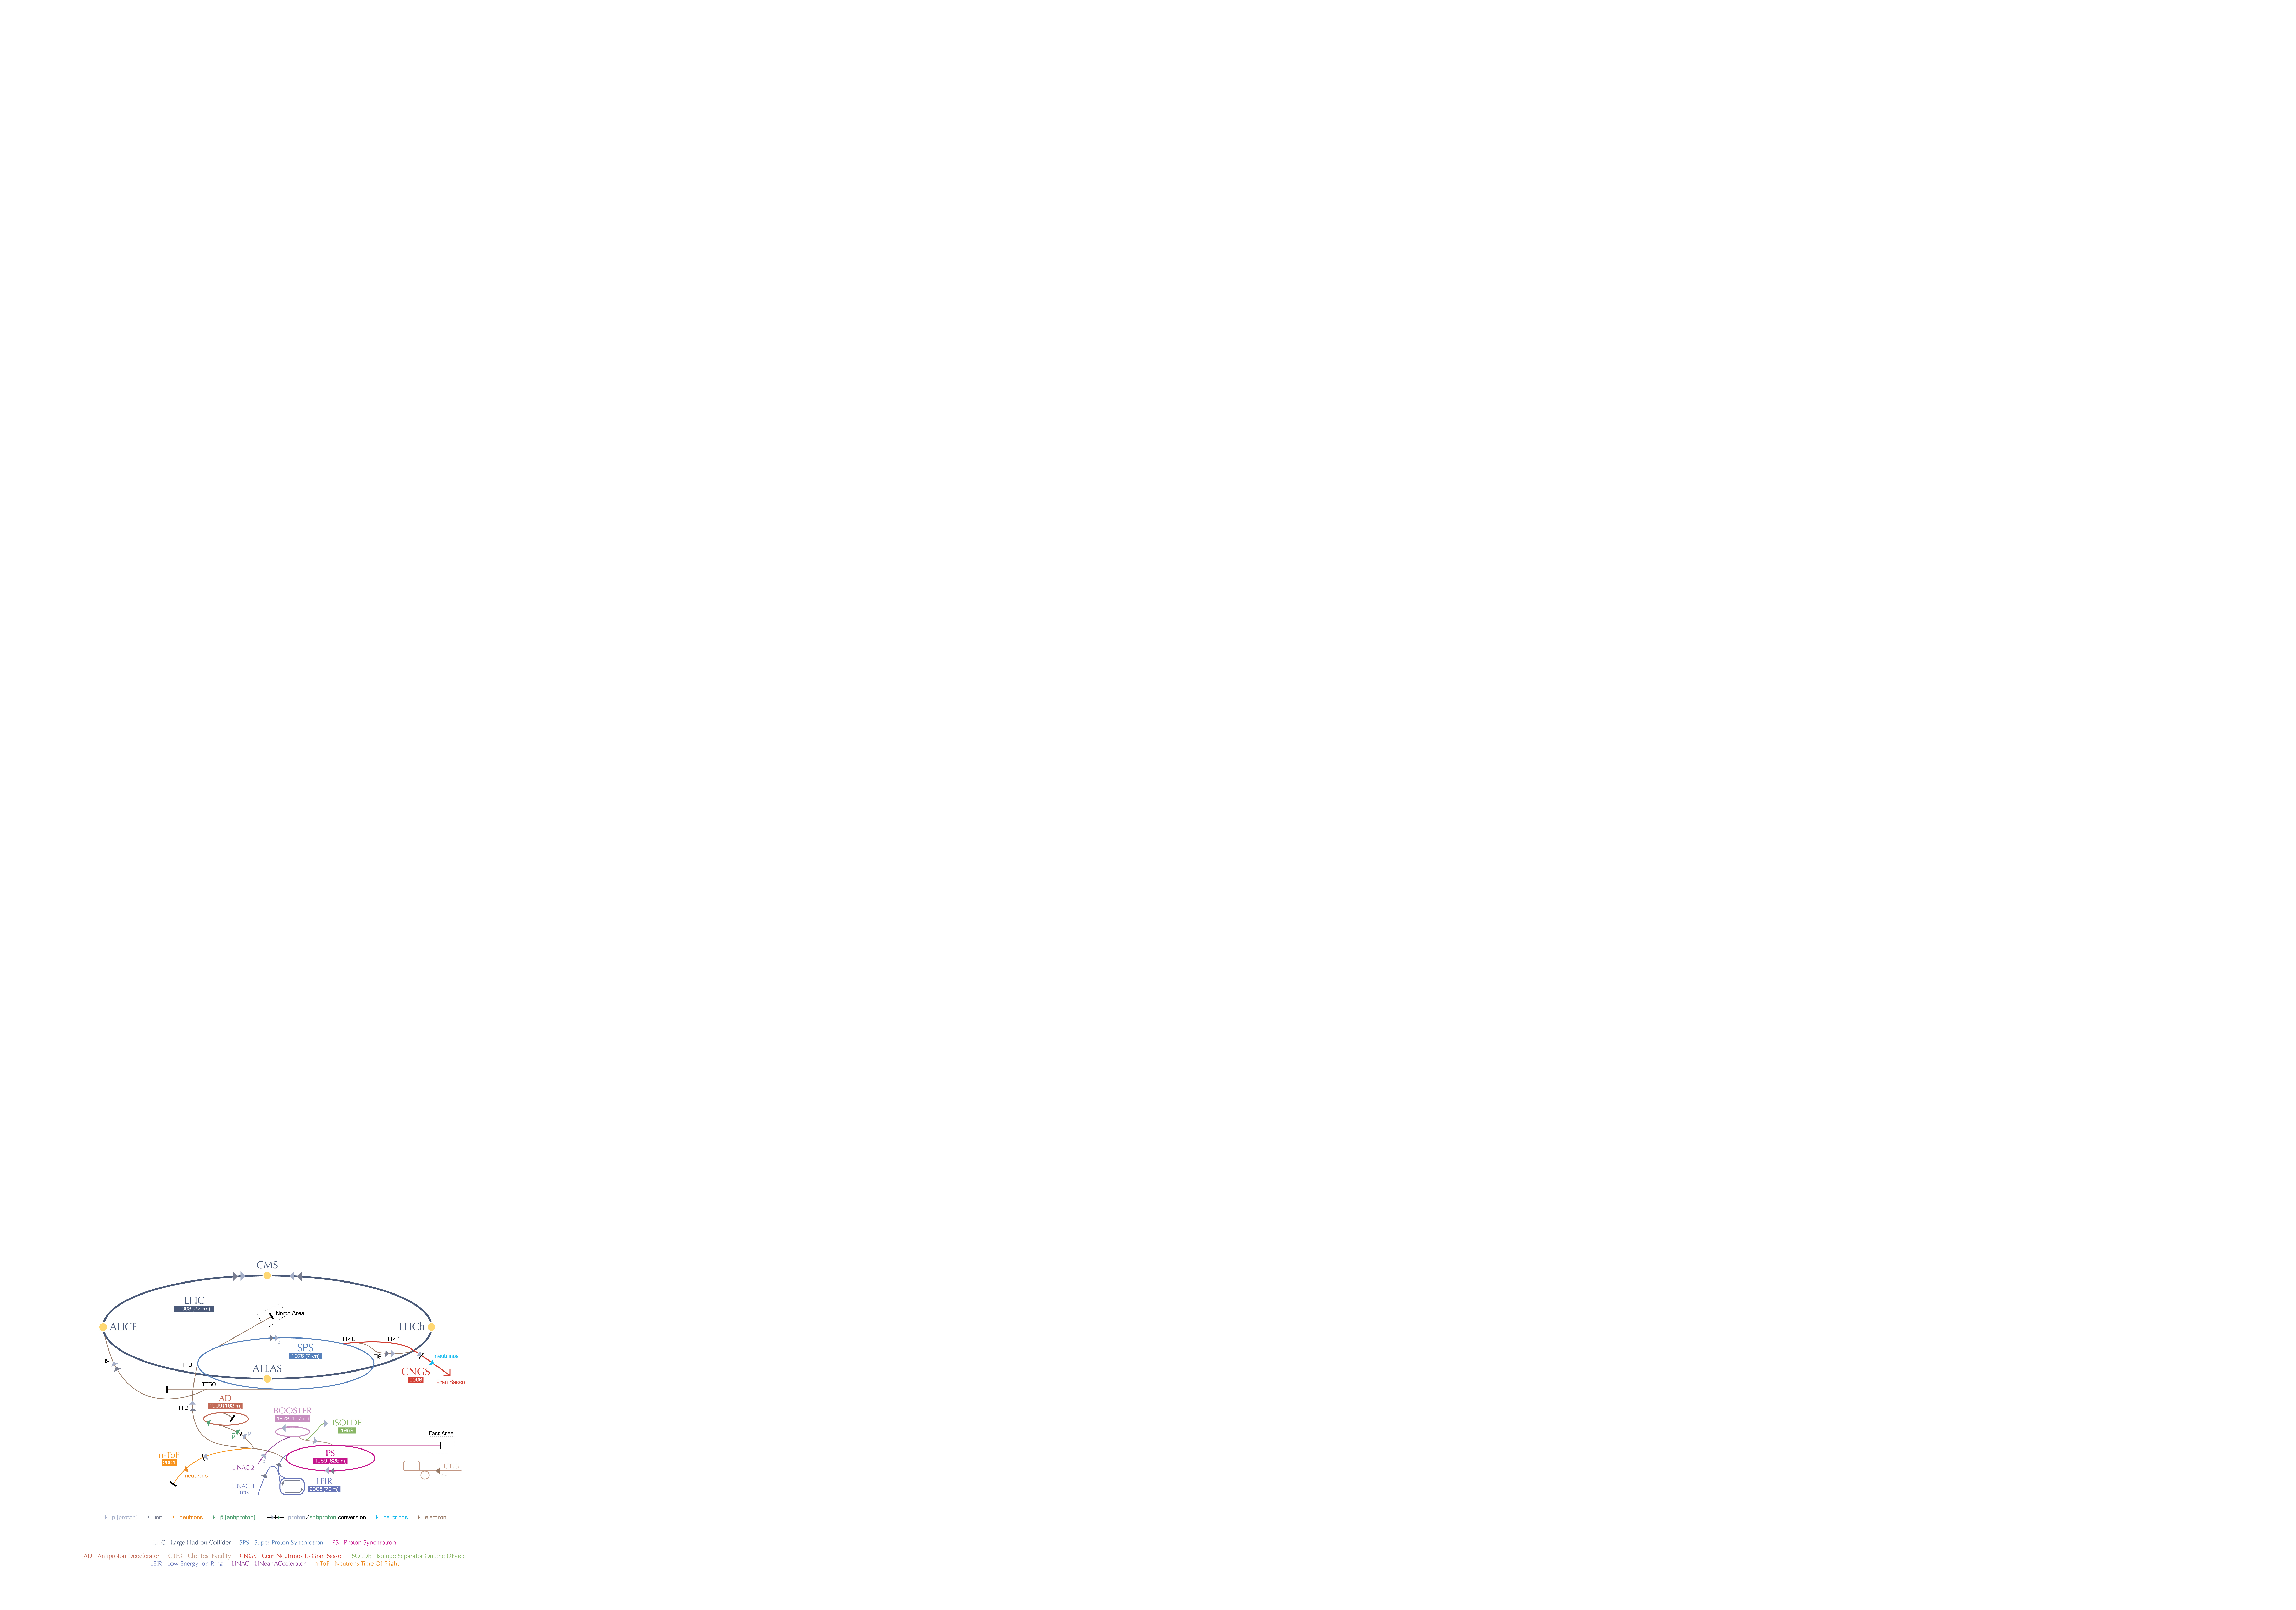
\includegraphics[width=\textwidth]{figures_and_tables/experimental_setup/lhc_complex.pdf}
    \caption{The LHC is the last ring (dark grey line) in a complex chain of particle accelerators. The smaller machines are used in a chain to help boost the particles to their final energies and provide beams to a whole set of smaller experiments. Source:~\cite{lhc_complex}.}
    \label{lhc_complex}
  \end{figure}